%----------------------------------------------------------
\chapter{Программная реализация}
\label{ch:chap3_soft_architecture}
%----------------------------------------------------------
\section{Архитектура}
\label{sec:architecture}

Изначально компилятор был написан на языке программирования Kotlin, однако было принято решение переписать его на другой язык - Rust.
Основные преимущества:
\begin{itemize}
    \item Rust работает быстрее, так как использует при компиляции llvm, что значит более хорошую оптимизацию, а так же применяет более строгие требования к разработке в целом,
    \item он предоставляет больше гарантий разработчику, как посредством его системы типов, так и другими средствами, например, borrow checker,
    \item система сборки создает нативный файл программы, в то время как система сборки Kotlin - файл, зависимый от JRE
\end{itemize}

Основной проблемой как раз и стало недостаточное количество гарантий во время компиляции и усложнение разработки из-за этого.
Даже если ошибка отлавливается с помощью проверок во время исполнения, её бывало трудно воспроизвести.

Отсюда и возникли дополнительные задачи по проектированию новой структуры AST программы, взаимодействием с этим деревом, а так же самым главным - разработке семантического анализатора.

Работать с большими проектами в разы удобнее при грамотном разбиении на модули.
В экосистеме Rust такие модули именуются крейтами (англ. crates).
На диаграмме ниже представлено разбиение на модули проекта Kodept.

\begin{figure}[H]
    \centering
    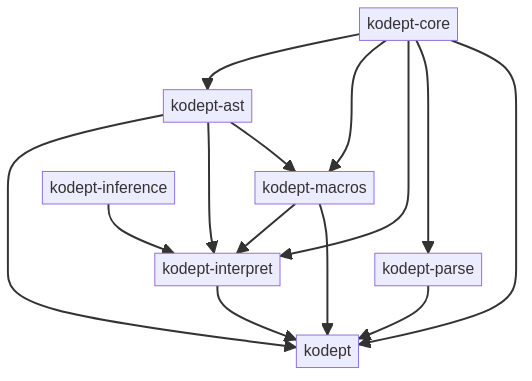
\includegraphics[width=0.75\textwidth]{figures/modules}
    \caption{Иерархия модулей в проекте}
    \label{fig:modules}
\end{figure}

%----------------------------------------------------------

